\documentclass{article}\usepackage[]{graphicx}\usepackage[]{color}
% maxwidth is the original width if it is less than linewidth
% otherwise use linewidth (to make sure the graphics do not exceed the margin)
\makeatletter
\def\maxwidth{ %
  \ifdim\Gin@nat@width>\linewidth
    \linewidth
  \else
    \Gin@nat@width
  \fi
}
\makeatother

\definecolor{fgcolor}{rgb}{0.345, 0.345, 0.345}
\newcommand{\hlnum}[1]{\textcolor[rgb]{0.686,0.059,0.569}{#1}}%
\newcommand{\hlstr}[1]{\textcolor[rgb]{0.192,0.494,0.8}{#1}}%
\newcommand{\hlcom}[1]{\textcolor[rgb]{0.678,0.584,0.686}{\textit{#1}}}%
\newcommand{\hlopt}[1]{\textcolor[rgb]{0,0,0}{#1}}%
\newcommand{\hlstd}[1]{\textcolor[rgb]{0.345,0.345,0.345}{#1}}%
\newcommand{\hlkwa}[1]{\textcolor[rgb]{0.161,0.373,0.58}{\textbf{#1}}}%
\newcommand{\hlkwb}[1]{\textcolor[rgb]{0.69,0.353,0.396}{#1}}%
\newcommand{\hlkwc}[1]{\textcolor[rgb]{0.333,0.667,0.333}{#1}}%
\newcommand{\hlkwd}[1]{\textcolor[rgb]{0.737,0.353,0.396}{\textbf{#1}}}%
\let\hlipl\hlkwb

\usepackage{framed}
\makeatletter
\newenvironment{kframe}{%
 \def\at@end@of@kframe{}%
 \ifinner\ifhmode%
  \def\at@end@of@kframe{\end{minipage}}%
  \begin{minipage}{\columnwidth}%
 \fi\fi%
 \def\FrameCommand##1{\hskip\@totalleftmargin \hskip-\fboxsep
 \colorbox{shadecolor}{##1}\hskip-\fboxsep
     % There is no \\@totalrightmargin, so:
     \hskip-\linewidth \hskip-\@totalleftmargin \hskip\columnwidth}%
 \MakeFramed {\advance\hsize-\width
   \@totalleftmargin\z@ \linewidth\hsize
   \@setminipage}}%
 {\par\unskip\endMakeFramed%
 \at@end@of@kframe}
\makeatother

\definecolor{shadecolor}{rgb}{.97, .97, .97}
\definecolor{messagecolor}{rgb}{0, 0, 0}
\definecolor{warningcolor}{rgb}{1, 0, 1}
\definecolor{errorcolor}{rgb}{1, 0, 0}
\newenvironment{knitrout}{}{} % an empty environment to be redefined in TeX

\usepackage{alltt}
%\usepackage{media9}



\title{Epidemiology -- Human and Water Borne Illnesses}
\author{Marc Los Huertos}
\IfFileExists{upquote.sty}{\usepackage{upquote}}{}
\begin{document}

\maketitle

COVID-19 began rapidly spreading around the world in late 2019. And by the spring, Italy went into lock down, California declared a state of emergency, schools and universities around the globe suspended in person classes and events, and businesses reduced travel and pushed tele-work policies. All of this was designed to slow the spread of the disease. These efforts are broadly referred to as social distancing.

\subsection{Value of Social Distancing}
The idea is to reduce person-to-person contact to make spreading the disease less likely. The effects of this are often illustrated in images such as those in the chart below, where the red plot is flattened to spread out the disease as much as possible. This helps to ensure that there are sufficient resources available for a sick population, which will help improve survival rates.

Flattening the curve to keep infection manageable (Source: Fast.ai).
How do we determine the value of such distancing strategies and model this spread?

\subsection{Modeling Disease -- SEIR}

We walk through a SEIR epidemiological model and simulate it with R. The first model is the basic SEIR without social distancing, then we add social distancing to show how the potential effectiveness of these strategies.

The SEIR model is a compartmental model for modeling how a disease spreads through a population. It's an acronym for Susceptible, Exposed, Infected, Recovered. When a disease is introduced to a population, the people move from one of these classes (or compartments) to the next. When they reach the R state, they're no longer able to be infected, depending on your interpretation, they either survived the disease and are now immune or succumbed to the illness and are out of the population.

This is an extension of the classic SIR model and simply adds one more equation to show those who are exposed. 


The Kermack-McKendrick model is an SIR model for the number of people infected with a contagious illness in a closed population over time. It was proposed to explain the rapid rise and fall in the number of infected patients observed in epidemics such as the plague (London 1665-1666, Bombay 1906) and cholera (London 1865). It assumes that the population size is fixed (i.e., no births, deaths due to disease, or deaths by natural causes), incubation period of the infectious agent is instantaneous, and duration of infectivity is same as length of the disease. It also assumes a completely homogeneous population with no age, spatial, or social structure.

The model consists of a system of three coupled nonlinear ordinary differential equations,


\begin{equation}
(dS)/(dt)	=	-\beta SI	
\end{equation}

\begin{equation}
(dI)/(dt)	=	\beta SI- \gamma I
\end{equation}

\begin{equation}
(dR)/(dt)	=	\gamma I,
\end{equation}

where t is time, S(t) is the number of susceptible people, I(t) is the number of people infected, R(t) is the number of people who have recovered and developed immunity to the infection, beta is the infection rate, and gamma is the recovery rate.

The key value governing the time evolution of these equations is the so-called epidemiological threshold,

\begin{equation}
 R_0=(\beta S)/ \gamma
\end{equation}
 
Note that the choice of the notation R\_0 is a bit unfortunate, since it has nothing to do with R. R\_0 is defined as the number of secondary infections caused by a single primary infection; in other words, it determines the number of people infected by contact with a single infected person before his death or recovery.The full model is given below:

We have four ODE's in the time domain, with three parameters: $\alpha$, $\beta$, $\gamma$.

\begin{itemize}

\item $\alpha$ is the inverse of the incubation period ($1/t_{incubation}$)
\item $\beta$ is the average contact rate in the population
\item $\gamma$ is the inverse of the mean infectious period ($1/t_{infectious}$)

\end{itemize}


Equation (1) is the change in people susceptible to the disease and is moderated by the number of infected people and their contact with the infected. Equation (2) gives the people who have been exposed to the disease. It grows based on the contact rate and decreases based on the incubation period whereby people then become infected.


\section{Models with Susceptibility and Infection}

\subsection{Model Structure}

The model relies on spatially explicit movements of 'subjects' that basically bounce around in a box, i.e. petri dish. Each subject is assigned a random location and trajectory (angle) of movement and velocity of movement vector. I based the model on an Washington Times article by XXXX (published). Although his model, written in Java, is probably much cleaner, I wanted to create something that students could use to adjust parameters and evaluate different policy strategies, using XX's visualization as a foundation. 

To track subject movements, contact with others, etc I have defined an array to track subject, thus, have to do some backflips to track overlap at each time step to see if people are sharing space and pathogens. 

I'm not a programmer, so this is going to need some TLC as it's pretty ineffecient. 

\subsection{Model Parameterization}



I have define the following parameters for the model, which will be further described in each section below.

% latex table generated in R 3.6.0 by xtable 1.8-4 package
% Fri Mar 20 11:03:07 2020
\begin{table}[ht]
\centering
\begin{tabular}{rlrrrrrrrrr}
  \hline
 & Model & N & Velocity & tstep & Stationary & Inf\_Dist & init\_infact & asymp & symp & rec \\ 
  \hline
1 & Model1 & 50.00 & 5.00 & 2000.00 & 0.00 & 20.00 & 2.00 & 24.00 & 96.00 & 720.00 \\ 
  2 & Model2 & 100.00 & 5.00 & 2000.00 & 0.00 & 20.00 & 2.00 & 24.00 & 96.00 & 720.00 \\ 
  3 & Model3 & 100.00 & 5.00 & 3000.00 & 0.40 & 20.00 & 2.00 & 24.00 & 96.00 & 720.00 \\ 
  4 & Model4 & 100.00 & 5.00 & 3000.00 & 0.40 & 20.00 & 2.00 & 60.00 & 60.00 & 720.00 \\ 
   \hline
\end{tabular}
\end{table}


But for now, I'd like to see how these align with the equations described above.

\subsection{Model Functions}

First, functions are useful when you have repetitive actions to make -- in this case, I have defined functions to move sujects based on their speed and direction of travel. 

Since these functions rely on the data array within another function (thus, not globally available, until it it `returned` at the end fo the function), I had to include a refernece to the data in the function so that the functions could find the array.

\begin{knitrout}
\definecolor{shadecolor}{rgb}{0.969, 0.969, 0.969}\color{fgcolor}\begin{kframe}
\begin{alltt}
\hlcom{#create function to move the subject}
\hlstd{move_x} \hlkwb{=} \hlkwa{function}\hlstd{(}\hlkwc{data_array}\hlstd{,} \hlkwc{s}\hlstd{,} \hlkwc{t}\hlstd{)\{}
\hlstd{data_array[s,} \hlnum{4}\hlstd{, t]} \hlopt{*} \hlkwd{cos}\hlstd{(data_array[s,}\hlnum{3}\hlstd{, t]}\hlopt{*}\hlstd{pi}\hlopt{/}\hlnum{180}\hlstd{)\}}
\hlstd{move_y} \hlkwb{=} \hlkwa{function}\hlstd{(}\hlkwc{data_array}\hlstd{,} \hlkwc{s}\hlstd{,} \hlkwc{t}\hlstd{)\{}
\hlstd{data_array[s,} \hlnum{4}\hlstd{, t]} \hlopt{*} \hlkwd{sin}\hlstd{(data_array[s,}\hlnum{3}\hlstd{, t]}\hlopt{*}\hlstd{pi}\hlopt{/}\hlnum{180}\hlstd{)\}}

\hlcom{# check function }
\hlcom{# move_y(data_arr, 1, 1); move_x(data_arr, 1,1)}

\hlcom{# move function}
\hlstd{move} \hlkwb{=} \hlkwa{function}\hlstd{(}\hlkwc{data_array}\hlstd{,} \hlkwc{s}\hlstd{,} \hlkwc{t}\hlstd{)\{}
  \hlkwd{c}\hlstd{(data_array[s,} \hlnum{1}\hlstd{, t}\hlopt{-}\hlnum{1}\hlstd{]}\hlopt{+} \hlkwd{move_x}\hlstd{(data_array, s, t}\hlopt{-}\hlnum{1}\hlstd{),}
    \hlstd{data_array[s,} \hlnum{2}\hlstd{, t}\hlopt{-}\hlnum{1}\hlstd{]}\hlopt{+} \hlkwd{move_y}\hlstd{(data_array, s, t}\hlopt{-}\hlnum{1}\hlstd{),}
    \hlstd{data_array[s,} \hlnum{3}\hlstd{, t}\hlopt{-}\hlnum{1}\hlstd{],}
    \hlstd{data_array[s,} \hlnum{4}\hlstd{, t}\hlopt{-}\hlnum{1}\hlstd{],}
    \hlstd{data_array[s,} \hlnum{5}\hlstd{, t}\hlopt{-}\hlnum{1}\hlstd{],}
    \hlstd{data_array[s,} \hlnum{6}\hlstd{, t}\hlopt{-}\hlnum{1}\hlstd{])}
\hlstd{\}}

\hlcom{# Test functions}
\hlcom{# data_arr[1,,1]}
\hlcom{# move(data_arr, 1, 2)}
\hlcom{# Model1; i = 2}
\end{alltt}
\end{kframe}
\end{knitrout}

\begin{knitrout}
\definecolor{shadecolor}{rgb}{0.969, 0.969, 0.969}\color{fgcolor}\begin{kframe}
\begin{alltt}
\hlcom{# Contact Infection Function}
\hlstd{contact} \hlkwb{=} \hlkwa{function}\hlstd{(}\hlkwc{data_array}\hlstd{,} \hlkwc{t}\hlstd{,} \hlkwc{Infect_dist}\hlstd{)\{}

\hlcom{# testfunction}
  \hlcom{#data_array=Model1_50; t=88; infect_dist = 5}
  \hlstd{pairs} \hlkwb{=} \hlkwd{cbind}\hlstd{(}\hlkwd{as.vector}\hlstd{(data_array[,}\hlstr{"x"}\hlstd{,t]),}
          \hlkwd{as.vector}\hlstd{(data_array[,}\hlstr{"y"}\hlstd{,t])); pairs}
  \hlstd{tmp} \hlkwb{=} \hlkwd{as.matrix}\hlstd{(}\hlkwd{dist}\hlstd{(pairs,} \hlkwc{method} \hlstd{=} \hlstr{"euclidean"} \hlstd{)); tmp}
  \hlstd{tmp[}\hlkwd{upper.tri}\hlstd{(tmp,} \hlkwc{diag} \hlstd{=} \hlnum{TRUE}\hlstd{)]} \hlkwb{<-} \hlnum{NA}\hlstd{; tmp}
  \hlstd{pairs} \hlkwb{<-} \hlkwd{which}\hlstd{(tmp} \hlopt{<} \hlstd{Infect_dist ,}\hlkwc{arr.ind} \hlstd{=} \hlnum{TRUE}\hlstd{);pairs}
  \hlstd{tmp2} \hlkwb{=} \hlkwd{cbind}\hlstd{(}\hlkwd{as.numeric}\hlstd{(}\hlkwd{rownames}\hlstd{(tmp)[pairs[,} \hlnum{1}\hlstd{]]),}
               \hlkwd{as.numeric}\hlstd{(}\hlkwd{colnames}\hlstd{(tmp)[pairs[,} \hlnum{2}\hlstd{]])); tmp2}
  \hlstd{contacts} \hlkwb{=} \hlkwd{dim}\hlstd{(tmp2)[}\hlnum{1}\hlstd{]; contacts}
  \hlkwa{if}\hlstd{(contacts}\hlopt{>}\hlnum{0}\hlstd{)\{}
    \hlkwa{for}\hlstd{(i} \hlkwa{in} \hlnum{1}\hlopt{:}\hlstd{contacts)\{}
      \hlcom{# If one is exposed, susceptable is exposed}
      \hlkwa{if}\hlstd{(data_array[tmp2[i,}\hlnum{1}\hlstd{],}\hlnum{5}\hlstd{,t]}\hlopt{==}\hlnum{2} \hlopt{&} \hlstd{data_array[tmp2[i,}\hlnum{2}\hlstd{],}\hlnum{5}\hlstd{,t]}\hlopt{==}\hlnum{1}\hlstd{)\{}
      \hlstd{data_array[tmp2[i,}\hlnum{2}\hlstd{],}\hlnum{5}\hlstd{,t]} \hlkwb{=} \hlnum{2}
      \hlstd{\}}
      \hlcom{# If one is exposed, susceptable is exposed}
      \hlkwa{if}\hlstd{(data_array[tmp2[i,}\hlnum{2}\hlstd{],}\hlnum{5}\hlstd{,t]}\hlopt{==}\hlnum{2} \hlopt{&} \hlstd{data_array[tmp2[i,}\hlnum{1}\hlstd{],}\hlnum{5}\hlstd{,t]}\hlopt{==}\hlnum{1}\hlstd{)\{}
      \hlstd{data_array[tmp2[i,}\hlnum{1}\hlstd{],}\hlnum{5}\hlstd{,t]} \hlkwb{=} \hlnum{2}
      \hlstd{\}}
      \hlcom{# If one is symptomatic, the susceptable is exposed}
      \hlkwa{if}\hlstd{(data_array[tmp2[i,}\hlnum{1}\hlstd{],}\hlnum{5}\hlstd{,t]}\hlopt{==}\hlnum{3} \hlopt{&} \hlstd{data_array[tmp2[i,}\hlnum{2}\hlstd{],}\hlnum{5}\hlstd{,t]}\hlopt{==}\hlnum{1}\hlstd{)\{}
      \hlstd{data_array[tmp2[i,}\hlnum{2}\hlstd{],} \hlnum{5}\hlstd{, t]} \hlkwb{=} \hlnum{2}
      \hlstd{\}}
      \hlcom{# If one is symptomatic, the susceptable is exposed}
      \hlkwa{if}\hlstd{(data_array[tmp2[i,}\hlnum{1}\hlstd{],}\hlnum{5}\hlstd{,t]}\hlopt{==}\hlnum{1} \hlopt{&} \hlstd{data_array[tmp2[i,}\hlnum{2}\hlstd{],}\hlnum{5}\hlstd{,t]}\hlopt{==}\hlnum{3}\hlstd{)\{}
      \hlstd{data_array[tmp2[i,}\hlnum{1}\hlstd{],} \hlnum{5}\hlstd{, t]} \hlkwb{=} \hlnum{2}
      \hlstd{\}}
    \hlstd{\}}

  \hlstd{\}}
   \hlcom{# data_array[,,t]}
\hlkwd{return}\hlstd{(data_array)}
\hlcom{# print(data_array[,5,t])}
\hlstd{\}} \hlcom{# close function}

\hlcom{#contact(Model1, 87, 5)}
\end{alltt}
\end{kframe}
\end{knitrout}

Next, I'm going to figure out how to create a function to text for euclidian distances to spread disease, but this will take some more effort \ldots

\subsection{Model 1: Modeling Susceptability and Infections  with No Behavior Changes and Recovery}

For this model, people get instantenously sick and start spreading it around -- not very realistic because when people get sick they are usually quarantined and stop bouncing around the environment. Nevertheless this sets up a good base line, where the poputation gets ill pretty quickly. 
\begin{knitrout}
\definecolor{shadecolor}{rgb}{0.969, 0.969, 0.969}\color{fgcolor}\begin{kframe}
\begin{alltt}
\hlstd{MoveSubjects} \hlkwb{=} \hlkwa{function}\hlstd{(}\hlkwc{N}\hlstd{=}\hlnum{3}\hlstd{,} \hlkwc{tstep}\hlstd{=}\hlnum{4}\hlstd{,} \hlkwc{Velocity} \hlstd{=} \hlnum{5}\hlstd{,} \hlkwc{Stationary} \hlstd{=} \hlnum{0}\hlstd{,} \hlkwc{Infect_dist} \hlstd{=} \hlnum{5}\hlstd{,} \hlkwc{Init_infect}\hlstd{=}\hlnum{1}\hlstd{,} \hlkwc{Speed}\hlstd{=}\hlnum{5}\hlstd{)\{}
\hlcom{# Test Defaults}
\hlcom{#N=3; tstep =4; Speed=5; Init_infect=1; stationary=.5}
\hlcom{# Define Data Array}
\hlstd{location} \hlkwb{=} \hlnum{6} \hlcom{# number of parameters to track}
\hlstd{data_arr} \hlkwb{=} \hlkwd{array}\hlstd{(}\hlkwc{dim}\hlstd{=}\hlkwd{c}\hlstd{(N, location, tstep))}
\hlkwd{dimnames}\hlstd{(data_arr)[[}\hlnum{2}\hlstd{]]} \hlkwb{<-} \hlkwd{c}\hlstd{(}\hlstr{"x"}\hlstd{,} \hlstr{"y"}\hlstd{,} \hlstr{"theta"}\hlstd{,} \hlstr{"velocity"}\hlstd{,} \hlstr{"status"}\hlstd{,} \hlstr{"count"}\hlstd{)}
\hlstd{data_arr[,,}\hlnum{1}\hlstd{]}
\hlcom{# Initialize Start Locations}
\hlkwd{set.seed}\hlstd{(}\hlnum{2763}\hlstd{)}
\hlstd{subj_x} \hlkwb{=} \hlkwd{runif}\hlstd{(N, coord_range[}\hlnum{1}\hlstd{],  coord_range[}\hlnum{2}\hlstd{]); subj_x}
\hlstd{subj_y} \hlkwb{=} \hlkwd{runif}\hlstd{(N, coord_range[}\hlnum{3}\hlstd{],  coord_range[}\hlnum{4}\hlstd{]); subj_y}

\hlcom{# Set Up Population Characteristics and Behaviors}
\hlstd{sheltered} \hlkwb{=} \hlkwd{sample}\hlstd{(N}\hlopt{*}\hlstd{Stationary); sheltered}
\hlstd{velocity} \hlkwb{=} \hlkwd{rep}\hlstd{(Velocity,N); velocity[sheltered]}\hlkwb{=}\hlnum{0}\hlstd{; velocity}
\hlstd{theta} \hlkwb{=} \hlkwd{round}\hlstd{(}\hlkwd{runif}\hlstd{(N,} \hlnum{0}\hlstd{,} \hlnum{360}\hlstd{),}\hlnum{0}\hlstd{); theta}
\hlstd{SEIR} \hlkwb{=} \hlkwd{rep}\hlstd{(}\hlnum{1}\hlstd{, N); SEIR[sheltered]} \hlkwb{=} \hlnum{0}
\hlstd{SEIR[}\hlkwd{sample}\hlstd{(N, Init_infect)]} \hlkwb{=} \hlnum{3}\hlstd{; SEIR}
\hlstd{count} \hlkwb{=} \hlkwd{rep}\hlstd{(}\hlnum{0}\hlstd{, N)}

\hlcom{# Initial Locations}
\hlstd{data_arr[,,}\hlnum{1}\hlstd{]} \hlkwb{=} \hlkwd{c}\hlstd{(subj_x, subj_y, theta, velocity, SEIR, count)}
\hlstd{data_arr[,,}\hlnum{1}\hlstd{]}
\hlcom{# t = 2; s=1}
\hlkwa{for}\hlstd{(t} \hlkwa{in} \hlnum{2}\hlopt{:}\hlstd{tstep)\{}
  \hlkwa{for}\hlstd{(s} \hlkwa{in} \hlnum{1}\hlopt{:}\hlstd{N)\{}
    \hlcom{# move subjects based on theta and speed}
    \hlstd{data_arr[s,,t]} \hlkwb{=} \hlkwd{move}\hlstd{(data_arr, s, t)}
    \hlcom{# coarse corrections when hitting a boundary}
    \hlcom{# Min x-boundary}
    \hlkwa{if}\hlstd{(data_arr[s,}\hlnum{1}\hlstd{,t]} \hlopt{<} \hlstd{coord_range[}\hlnum{1}\hlstd{])\{}
      \hlstd{data_arr[s,}\hlnum{3}\hlstd{,t}\hlopt{-}\hlnum{1}\hlstd{]}\hlkwb{=}\hlnum{180}\hlopt{-}\hlstd{data_arr[s,}\hlnum{3}\hlstd{,t}\hlopt{-}\hlnum{1}\hlstd{]}
      \hlstd{data_arr[s,,t]} \hlkwb{=} \hlkwd{move}\hlstd{(data_arr, s, t)}
    \hlstd{\}}
    \hlcom{#Max x-boundary}
    \hlkwa{if}\hlstd{(data_arr[s,}\hlnum{1}\hlstd{,t]} \hlopt{>} \hlstd{coord_range[}\hlnum{2}\hlstd{])\{}
      \hlstd{data_arr[s,}\hlnum{3}\hlstd{,t}\hlopt{-}\hlnum{1}\hlstd{]}\hlkwb{=}\hlnum{180}\hlopt{-}\hlstd{data_arr[s,}\hlnum{3}\hlstd{,t}\hlopt{-}\hlnum{1}\hlstd{]}
      \hlstd{data_arr[s,,t]} \hlkwb{=} \hlkwd{move}\hlstd{(data_arr, s, t)}
    \hlstd{\}}
    \hlcom{#Min y-boundary}
    \hlkwa{if}\hlstd{(data_arr[s,}\hlnum{2}\hlstd{,t]} \hlopt{<} \hlstd{coord_range[}\hlnum{3}\hlstd{])\{}
      \hlstd{data_arr[s,}\hlnum{3}\hlstd{,t}\hlopt{-}\hlnum{1}\hlstd{]}\hlkwb{=}\hlnum{360}\hlopt{-}\hlstd{data_arr[s,}\hlnum{3}\hlstd{,t}\hlopt{-}\hlnum{1}\hlstd{]}
      \hlstd{data_arr[s,,t]} \hlkwb{=} \hlkwd{move}\hlstd{(data_arr, s, t)}
    \hlstd{\}}
    \hlcom{#Max y-boundary}
    \hlkwa{if}\hlstd{(data_arr[s,}\hlnum{2}\hlstd{,t]} \hlopt{>} \hlstd{coord_range[}\hlnum{4}\hlstd{])\{}
      \hlstd{data_arr[s,}\hlnum{3}\hlstd{,t}\hlopt{-}\hlnum{1}\hlstd{]}\hlkwb{=}\hlnum{360}\hlopt{-}\hlstd{data_arr[s,}\hlnum{3}\hlstd{,t}\hlopt{-}\hlnum{1}\hlstd{]}
      \hlstd{data_arr[s,,t]} \hlkwb{=} \hlkwd{move}\hlstd{(data_arr, s, t)}
    \hlstd{\}}
    \hlcom{# Change Status based on Time Steps}
    \hlstd{data_arr[s,}\hlnum{6}\hlstd{,t]} \hlkwb{=} \hlstd{data_arr[s,}\hlnum{6}\hlstd{,t]} \hlopt{+} \hlnum{1}
    \hlkwa{if}\hlstd{(data_arr[s,}\hlnum{5}\hlstd{,t]}\hlopt{==}\hlnum{1} \hlopt{|} \hlstd{data_arr[s,}\hlnum{5}\hlstd{,t]}\hlopt{==}\hlnum{0}\hlstd{) data_arr[s,}\hlnum{6}\hlstd{,t]}\hlkwb{=}\hlnum{0} \hlcom{# Reset Susceptables  }
   \hlcom{# Exposed becomes symptomatic}
  \hlkwa{if}\hlstd{(data_arr[s,}\hlnum{5}\hlstd{,t]}\hlopt{==}\hlnum{2} \hlopt{&} \hlstd{data_arr[s,}\hlnum{6}\hlstd{,t]} \hlopt{>} \hlstd{params[}\hlnum{1}\hlstd{,}\hlnum{6}\hlstd{])\{}
    \hlstd{data_arr[s,}\hlnum{5}\hlstd{,t]}\hlkwb{=}\hlnum{3}\hlstd{\}}
    \hlcom{# Symptomatics move very little}
  \hlkwa{if}\hlstd{(data_arr[s,}\hlnum{5}\hlstd{,t]}\hlopt{==}\hlnum{3} \hlopt{&} \hlstd{data_arr[s,}\hlnum{6}\hlstd{,t]} \hlopt{>} \hlstd{params[}\hlnum{1}\hlstd{,}\hlnum{7}\hlstd{])\{}
    \hlstd{data_arr[s,}\hlnum{4}\hlstd{,t]} \hlkwb{=} \hlnum{1}\hlstd{\}}
  \hlcom{# Time to Recovery}
  \hlkwa{if}\hlstd{(data_arr[s,}\hlnum{5}\hlstd{,t]}\hlopt{==}\hlnum{3} \hlopt{&} \hlstd{data_arr[s,}\hlnum{6}\hlstd{,t]} \hlopt{>} \hlstd{params[}\hlnum{1}\hlstd{,}\hlnum{8}\hlstd{])\{}
    \hlstd{data_arr[s,}\hlnum{5}\hlstd{,t]} \hlkwb{=} \hlnum{4}
    \hlstd{data_arr[s,}\hlnum{4}\hlstd{,t]} \hlkwb{=} \hlnum{5}
    \hlstd{\}}
  \hlstd{\}} \hlcom{# End of Subj Moving}

  \hlcom{# Time Step Proceesing}
  \hlcom{# Test for Euclidean Distances Here!}

\hlstd{data_arr} \hlkwb{<-} \hlkwd{contact}\hlstd{(data_arr, t, Infect_dist)}

\hlstd{\}} \hlcom{# End of Time Step}
\hlkwd{return}\hlstd{(data_arr)}
\hlstd{\}}
\end{alltt}
\end{kframe}
\end{knitrout}

\subsection{Model Runs}

For after running the models, I visually evaluated the models to make sure there weren't unintended consequences, i.e. usually from coding errors. Below are the models that I ran and the estimated run times. 

\begin{knitrout}
\definecolor{shadecolor}{rgb}{0.969, 0.969, 0.969}\color{fgcolor}\begin{kframe}
\begin{alltt}
\hlkwd{library}\hlstd{(tictoc)}
\hlcom{#N=3, tstep=4, speed=5, init_infect=1, stationary = 0)}
\hlstd{params}

\hlstd{m}\hlkwb{=}\hlnum{1}
\hlkwd{tic}\hlstd{(}\hlstr{"Model1"}\hlstd{)}
\hlstd{Model1}\hlkwb{<-} \hlkwd{MoveSubjects}\hlstd{(}\hlkwc{N} \hlstd{= params[m,}\hlnum{2}\hlstd{],} \hlkwc{Velocity} \hlstd{= params[m,} \hlnum{3}\hlstd{],}
    \hlkwc{tstep} \hlstd{= params[m,}\hlnum{4}\hlstd{],} \hlkwc{Stationary} \hlstd{= params[m,}\hlnum{5}\hlstd{],}
    \hlkwc{Infect_dist}\hlstd{=params[m,} \hlnum{6}\hlstd{],} \hlkwc{Init_infect}\hlstd{=params[m,} \hlnum{7}\hlstd{])}
\hlkwd{toc}\hlstd{()} \hlcom{# 900s}

\hlstd{m}\hlkwb{=}\hlnum{2}
\hlkwd{tic}\hlstd{(}\hlstr{"Model2"}\hlstd{)}
\hlstd{Model2}\hlkwb{<-} \hlkwd{MoveSubjects}\hlstd{(}\hlkwc{N} \hlstd{= params[m,}\hlnum{2}\hlstd{],} \hlkwc{Velocity} \hlstd{= params[m,} \hlnum{3}\hlstd{],}
    \hlkwc{tstep} \hlstd{= params[m,}\hlnum{4}\hlstd{],} \hlkwc{Stationary} \hlstd{= params[m,}\hlnum{5}\hlstd{],}
    \hlkwc{Infect_dist}\hlstd{=params[m,} \hlnum{6}\hlstd{],} \hlkwc{Init_infect}\hlstd{=params[m,} \hlnum{7}\hlstd{])}
\hlkwd{toc}\hlstd{()} \hlcom{#1800s}

\hlstd{m}\hlkwb{=}\hlnum{3}
\hlkwd{tic}\hlstd{(}\hlstr{"Model3"}\hlstd{)}
\hlstd{Model3} \hlkwb{<-} \hlkwd{MoveSubjects}\hlstd{(}\hlkwc{N} \hlstd{= params[m,}\hlnum{2}\hlstd{],} \hlkwc{Velocity} \hlstd{= params[m,} \hlnum{3}\hlstd{],}
    \hlkwc{tstep} \hlstd{= params[m,}\hlnum{4}\hlstd{],} \hlkwc{Stationary} \hlstd{= params[m,}\hlnum{5}\hlstd{],}
    \hlkwc{Infect_dist}\hlstd{=params[m,} \hlnum{6}\hlstd{],} \hlkwc{Init_infect}\hlstd{=params[m,} \hlnum{7}\hlstd{])}
\hlkwd{toc}\hlstd{()} \hlcom{#3308}

\hlstd{m}\hlkwb{=}\hlnum{4}
\hlkwd{tic}\hlstd{(}\hlstr{"Model4"}\hlstd{)}
\hlstd{Model4} \hlkwb{<-} \hlkwd{MoveSubjects}\hlstd{(}\hlkwc{N} \hlstd{= params[m,}\hlnum{2}\hlstd{],} \hlkwc{Velocity} \hlstd{= params[m,} \hlnum{3}\hlstd{],}
    \hlkwc{tstep} \hlstd{= params[m,}\hlnum{4}\hlstd{],} \hlkwc{Stationary} \hlstd{= params[m,}\hlnum{5}\hlstd{],}
    \hlkwc{Infect_dist}\hlstd{=params[m,} \hlnum{6}\hlstd{],} \hlkwc{Init_infect}\hlstd{=params[m,} \hlnum{7}\hlstd{])}
\hlkwd{toc}\hlstd{()} \hlcom{#3308}
\end{alltt}
\end{kframe}
\end{knitrout}

\subsection{Tracking the Disease Transfer}

\begin{knitrout}
\definecolor{shadecolor}{rgb}{0.969, 0.969, 0.969}\color{fgcolor}\begin{kframe}
\begin{alltt}
\hlcom{#load("/home/CAMPUS/mwl04747/github/beginnersluck.RData")}
\hlcom{# Susceptable 1, Exposed-Asymptomatic 2, Symptomatic 3, Recovered 4}
\hlstd{SEIRcol} \hlkwb{=} \hlkwd{c}\hlstd{(}\hlstr{"steelblue"}\hlstd{,} \hlstr{"orange"}\hlstd{,}\hlstr{"red"}\hlstd{,} \hlstr{"green"}\hlstd{)}

\hlstd{trackresults}\hlkwb{=}\hlkwa{function}\hlstd{(}\hlkwc{model}\hlstd{,}\hlkwc{m}\hlstd{,}\hlkwc{tstep}\hlstd{)\{}
\hlstd{results} \hlkwb{=} \hlkwd{data.frame}\hlstd{(}\hlkwc{Days} \hlstd{=} \hlnum{NA}\hlstd{,} \hlkwc{Sh} \hlstd{=} \hlnum{NA}\hlstd{,} \hlkwc{S}\hlstd{=}\hlnum{NA}\hlstd{,} \hlkwc{E}\hlstd{=}\hlnum{NA}\hlstd{,} \hlkwc{I}\hlstd{=}\hlnum{NA}\hlstd{,} \hlkwc{R}\hlstd{=}\hlnum{NA}\hlstd{)}
\hlkwa{for}\hlstd{(t} \hlkwa{in} \hlnum{1}\hlopt{:}\hlstd{tstep)\{}
\hlstd{days} \hlkwb{=} \hlstd{t}\hlopt{/}\hlnum{24}
\hlstd{sh} \hlkwb{=} \hlkwd{sum}\hlstd{(}\hlkwd{as.vector}\hlstd{(model[,}\hlnum{5}\hlstd{,t])}\hlopt{==}\hlnum{0}\hlstd{)}
\hlstd{s} \hlkwb{=} \hlkwd{sum}\hlstd{(}\hlkwd{as.vector}\hlstd{(model[,}\hlnum{5}\hlstd{,t])}\hlopt{==}\hlnum{1}\hlstd{, sh)}
\hlstd{e} \hlkwb{=} \hlkwd{sum}\hlstd{(}\hlkwd{as.vector}\hlstd{(model[,}\hlnum{5}\hlstd{,t])}\hlopt{==}\hlnum{2}\hlstd{)}
\hlstd{i} \hlkwb{=} \hlkwd{sum}\hlstd{(}\hlkwd{as.vector}\hlstd{(model[,}\hlnum{5}\hlstd{,t])}\hlopt{==}\hlnum{3}\hlstd{)}
\hlstd{r} \hlkwb{=} \hlkwd{sum}\hlstd{(}\hlkwd{as.vector}\hlstd{(model[,}\hlnum{5}\hlstd{,t])}\hlopt{==}\hlnum{4}\hlstd{)}
\hlstd{results[t,]} \hlkwb{<-} \hlkwd{data.frame}\hlstd{(}\hlkwc{Days} \hlstd{= days,} \hlkwc{Sh} \hlstd{= sh,} \hlkwc{S}\hlstd{=s,} \hlkwc{E}\hlstd{=e,} \hlkwc{I}\hlstd{=i,} \hlkwc{R}\hlstd{=r)}
\hlstd{\}}
\hlkwd{head}\hlstd{(results)}
\hlkwd{par}\hlstd{(}\hlkwc{mfrow}\hlstd{=}\hlkwd{c}\hlstd{(}\hlnum{1}\hlstd{,}\hlnum{1}\hlstd{),} \hlkwc{mar}\hlstd{=}\hlkwd{c}\hlstd{(}\hlnum{4}\hlstd{,} \hlnum{5}\hlstd{,} \hlnum{3}\hlstd{,} \hlnum{2}\hlstd{)}\hlopt{+}\hlnum{.1}\hlstd{,} \hlkwc{las}\hlstd{=}\hlnum{1}\hlstd{)}
\hlkwd{plot}\hlstd{(S}\hlopt{~}\hlstd{Days,} \hlkwc{data}\hlstd{=results,} \hlkwc{ty}\hlstd{=}\hlstr{'l'}\hlstd{,} \hlkwc{col}\hlstd{=SEIRcol[}\hlnum{1}\hlstd{],} \hlkwc{ylab}\hlstd{=}\hlstr{""}\hlstd{,} \hlkwc{ylim}\hlstd{=}\hlkwd{c}\hlstd{(}\hlnum{0}\hlstd{,params[m,}\hlnum{2}\hlstd{]),} \hlkwc{xlab}\hlstd{=}\hlstr{"Days"}\hlstd{,} \hlkwc{xlim}\hlstd{=}\hlkwd{c}\hlstd{(}\hlnum{0}\hlstd{,tstep}\hlopt{/}\hlnum{24}\hlstd{),} \hlkwc{lwd}\hlstd{=}\hlnum{2}\hlstd{,} \hlkwc{main} \hlstd{=} \hlkwd{paste}\hlstd{(params[m,} \hlnum{1}\hlstd{],} \hlstr{", Stationary ="}\hlstd{, params[m,}\hlnum{4}\hlstd{]}\hlopt{*}\hlnum{100}\hlstd{,} \hlstr{"%"}\hlstd{))}
\hlkwd{lines}\hlstd{(E}\hlopt{~}\hlstd{Days,} \hlkwc{data}\hlstd{=results,} \hlkwc{col}\hlstd{=SEIRcol[}\hlnum{2}\hlstd{],} \hlkwc{lwd}\hlstd{=}\hlnum{2}\hlstd{)}
\hlkwd{lines}\hlstd{(I}\hlopt{~}\hlstd{Days,} \hlkwc{data}\hlstd{=results,} \hlkwc{col}\hlstd{=SEIRcol[}\hlnum{3}\hlstd{],} \hlkwc{lwd}\hlstd{=}\hlnum{2}\hlstd{)}
\hlkwd{lines}\hlstd{(R}\hlopt{~}\hlstd{Days,} \hlkwc{data}\hlstd{=results,} \hlkwc{col}\hlstd{=SEIRcol[}\hlnum{4}\hlstd{],} \hlkwc{lwd}\hlstd{=}\hlnum{2}\hlstd{)}
\hlstd{\}}

\hlkwd{png}\hlstd{(}\hlkwc{filename} \hlstd{=}
  \hlstr{"/home/CAMPUS/mwl04747/github/beginnersluck/Epidemiology/Model1.png"}\hlstd{);}
  \hlstd{m} \hlkwb{=} \hlnum{1}\hlstd{;} \hlkwd{trackresults}\hlstd{(Model1, m, params[m,}\hlnum{3}\hlstd{]);} \hlkwd{dev.off}\hlstd{()}
\hlkwd{png}\hlstd{(}\hlkwc{filename} \hlstd{=}
  \hlstr{"/home/CAMPUS/mwl04747/github/beginnersluck/Epidemiology/Model2.png"}\hlstd{);}
  \hlstd{m} \hlkwb{=} \hlnum{2}\hlstd{;} \hlkwd{trackresults}\hlstd{(Model2, m, params[m,}\hlnum{3}\hlstd{]);} \hlkwd{dev.off}\hlstd{()}
\hlkwd{png}\hlstd{(}\hlkwc{filename} \hlstd{=}
  \hlstr{"/home/CAMPUS/mwl04747/github/beginnersluck/Epidemiology/Model3.png"}\hlstd{);}
  \hlstd{m} \hlkwb{=} \hlnum{3}\hlstd{;} \hlkwd{trackresults}\hlstd{(Model3, m, params[m,}\hlnum{3}\hlstd{]);} \hlkwd{dev.off}\hlstd{()}
\hlkwd{png}\hlstd{(}\hlkwc{filename} \hlstd{=}
  \hlstr{"/home/CAMPUS/mwl04747/github/beginnersluck/Epidemiology/Model4.png"}\hlstd{);}
  \hlstd{m} \hlkwb{=} \hlnum{4}\hlstd{;} \hlkwd{trackresults}\hlstd{(Model4, m, params[m,}\hlnum{3}\hlstd{]); dev.off}
\end{alltt}
\end{kframe}
\end{knitrout}

\begin{figure}
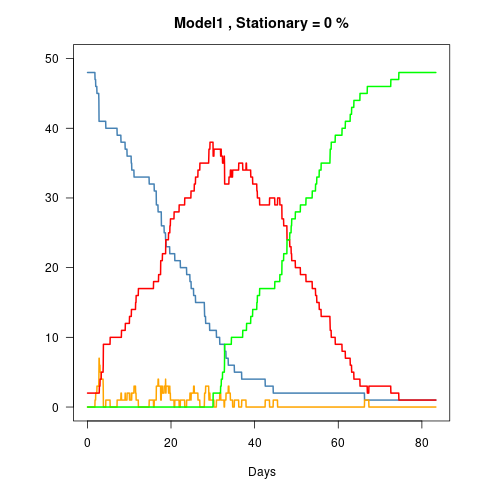
\includegraphics[width=1\textwidth]{Model1.png}
\caption{N = 50}
\end{figure}

\begin{figure}
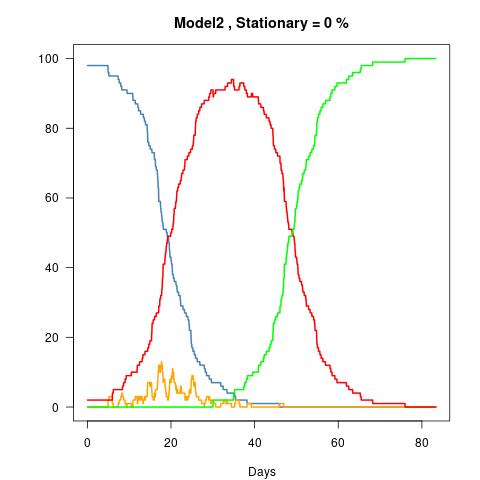
\includegraphics[width=1\textwidth]{Model2.png}
\caption{N=100}
\end{figure}

\begin{figure}
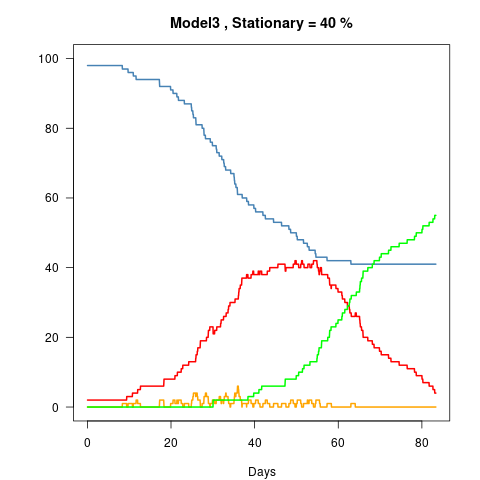
\includegraphics[width=1\textwidth]{Model3.png}
\caption{40\% shelter in place}
\end{figure}

\begin{figure}
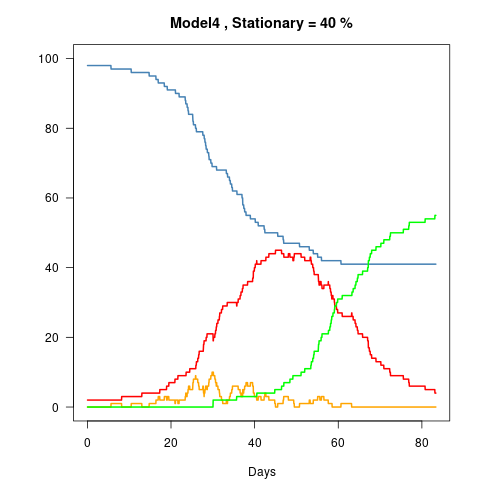
\includegraphics[width=1\textwidth]{Model4.png}
\caption{40\% shelter in place, exposed without symptoms.}
\end{figure}

\section{Plot Results}

\subsection{Static plot}

Because we are looking at a dynamic system, I don't find the static plot all that useful.



\begin{figure}
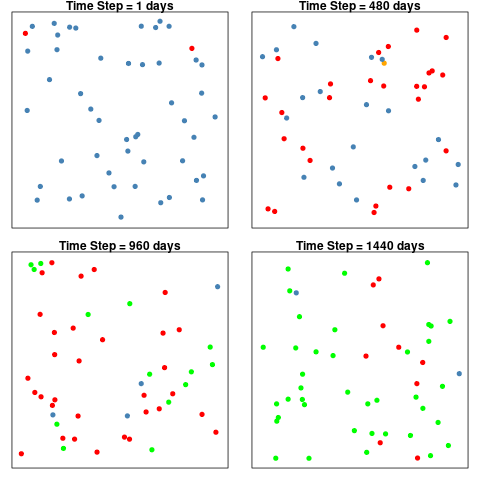
\includegraphics[width=1\textwidth]{SSModel1.png}
\caption{N = 50}
\end{figure}

\begin{figure}
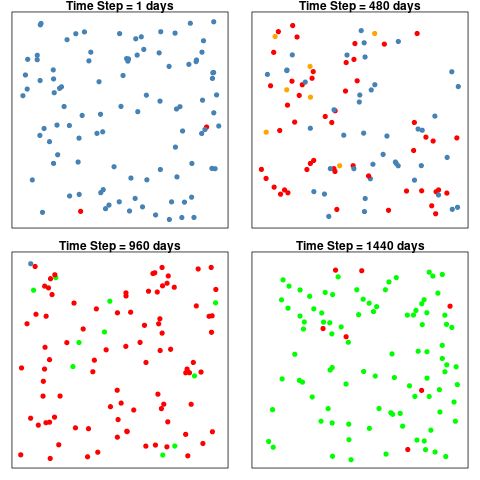
\includegraphics[width=1\textwidth]{SSModel2.png}
\caption{N=100}
\end{figure}

\begin{figure}
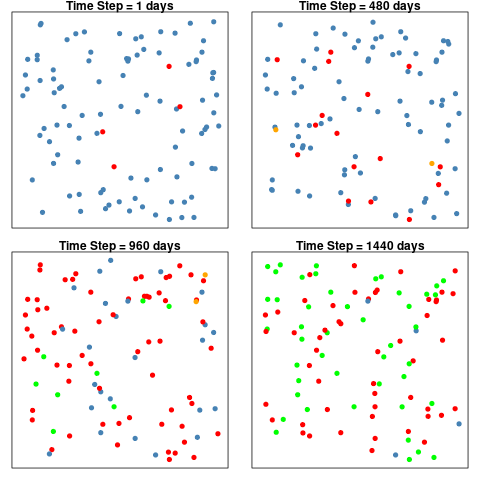
\includegraphics[width=1\textwidth]{SSModel3.png}
\caption{40\% shelter in place}
\end{figure}

\begin{figure}
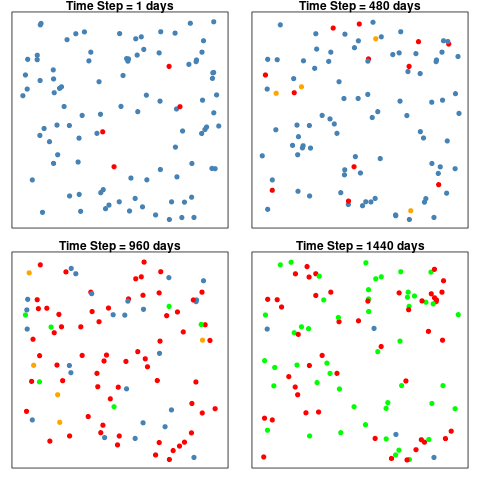
\includegraphics[width=1\textwidth]{SSModel4.png}
\caption{40\% shelter in place, exposed without symptoms.}
\end{figure}
\subsection{Animating the Results}

Still working on this... I have to export the file to my laptop then use photoshop to make a movie.

it would be nice to do this in r and then embedd in a pdf...



\end{document}
